%        File: !comp!expand("%:p:t")!comp!
%     Created: !comp!strftime("%a %b %d %I:00 %p %Y ").substitute(strftime('%Z'), '\<\(\w\)\(\w*\)\>\(\W\|$\)', '\1', 'g')!comp!
% Last Change: !comp!strftime("%a %b %d %I:00 %p %Y ").substitute(strftime('%Z'), '\<\(\w\)\(\w*\)\>\(\W\|$\)', '\1', 'g')!comp!
%
\documentclass[a4paper]{report} % report because I feel like I really need chapters formatting
\usepackage{listings}
\usepackage{amsmath,amssymb}
\usepackage{tikz}
\renewcommand{\thesection}{\arabic{section}}
\renewcommand{\thesubsection}{\thesection.\alph{subsection}}
\title{Tema 1 Algoritmi Avansati}
\author{Sociu Daniel}
\begin{document}
\maketitle

\tableofcontents

\chapter*{Knapsack}
\addcontentsline{toc}{chapter}{Knapsack}

\section{Problema 1}

\subsection{}
E nevoie doar de un simplu algoritm similar cu knapsack pseudo-polinomial, doar ca valoarea si greutatea sunt egale.

\lstinputlisting[language=C]{./knapsack/knapsack_a.cpp}

\subsection{}
Acest algoritm este cel putin 2*OPT in O(n) deoarece daca avem o suma care trece de K,
suma pe care o avem pana acum sau elementul care incercam sa il adunam, este mai mare de K/2
si doar selectam elementul mai mare. \newline

\lstinputlisting[language=C]{./knapsack/knapsack_b.cpp}

\chapter*{Load Balance}
\addcontentsline{toc}{chapter}{Load Balance}
\setcounter{section}{0}
\section{Problema 1}
Fie M1 si M2 lista job-urilor incarcate pe masina 1, respectiv masina 2

\subsection{}
Pentru a demonstra ca afirmatia e posibila sa fie adevarata, trebuie sa gasim minim un caz pe care e adevarata:

Sa presupunem masinile cu job-urile:

$M_{1}=\{80\}$

$M_{2}=\{80,40\}$

Observam ca $ALG=OPT \implies ALG\leq1.1*OPT$ deci afirmatia lui poate fi adevarata

\subsection{}
Pentru a demonstra ca afirmatia e false, aratam ca nu e exista un caz pentru care ar putea fi adevarata

Considerand multimea job-urile J si stiind $\forall x_{i} \in J, x_{i}\leq10$, observam ca diferenta maxima in $OPT$ va fi 10,
altfel o masina ar fi avut prea multa incarcatura, si ar exista o aranajare a job-urilor mai optima. Deci: \newline

$OPT\leq \max\{95,105\} \leq 105$ (105 e val maxima pt $OPT$)

Dar in cazul nostru:

$ALG= \max\{80,120\}=120 \implies 1.1*OPT=1.1*105\approx116\leq ALG=120$ Ceea ce e fals, adica e imposibil ca algoritmul sa fie $1.1*OPT$

\section{Problema 3}
Din curs stim:

Lema 1. \[OPT\geq \max\{\frac{1}{m} \sum_{1\leq i \leq n} t_{j} , \max\{t_{j} \mid 1\leq j \leq n\} \}\]

Si stim ca $ALG\leq \frac{3}{2}OPT$

Fie $K$ indicele masinii cu load-ul maxim la finalul algoritmului.

Fie $q$ ultimul job adaugat masinii $K$

Este evident ca algoritmul e optim in cazul in care sunt mai putine job-uri decat numarul masinilor, deci consideram cazul cand  avem mai mult de m job-uri

Fie $load'(M)$ load-ul masinii dupa ce am adaugat primele $q-1$ job-uri dar nu si job-ul $q$

O observatie importanta este ca $load'(K)$ este minimul dintre toate masinile si $load(K)=load'(K)+t(q)$, deci:

\[ALG=load(K)=load'(K)+t_{q}\leq \frac{1}{m}\sum_{i=1}^{m}load'(i)+t_{q}=\frac{1}{m}\sum_{i=1}^{q-1}t_{i}+t_{q} \]

Observam ca $t_{q}\leq \frac{1}{2}(t_{m} + t_{m+1})\leq OPT$ deoarece job-urile sunt sortate descrescator, deci ultimul job este mai mic sau egal cu media a 2 job-uri precedente. Deci:

\[\frac{1}{m}\sum_{i=1}^{q-1}t_{i} + t_{q} \leq \frac{1}{m}(\sum_{i=1}^{n}t_{i} - t_{q}) + \frac{1}{2}(t_{m}+t_{m+1})\leq \frac{1}{m}\sum_{i=1}^{n}t_{i}-\frac{1}{2\cdot m}(t_{m}+t_{m+1})+\frac{1}{2}(t_{m}+t_{m+1})\leq\]
Inlocuim cu $OPT$
\[\implies \leq OPT-\frac{1}{2\cdot m}OPT + \frac{1}{2}OPT = \frac{3}{2}OPT - \frac{1}{2\cdot m}OPT = (\frac{3}{2}-\frac{1}{2\cdot m})OPT\]

Deci avem ca:\[ALG\leq (\frac{3}{2}-\frac{1}{2\cdot m})OPT\]

\chapter*{TSP}
\addcontentsline{toc}{chapter}{TSP}
\setcounter{section}{0}
\section{Problema 1}
TSP unde muchiile au ponderea 1 sau 2. 

Sa pp. ca $\exists$ un algoritm polinomial si aproximativ $ALG\leq cOPT$ unde OPT e o rezolvare optima pentru TSP.

\subsection{}

Fie $G$ graful cu n noduri si ponderi 1 si 2 $\rightarrow$ observam ca $OPT$ e maxim $2n$.

Stim ca problema determinarii unui HC in G este NPC.

Construim $G'$ complet, muchiile comune intre $G$ si $G'$ isi pastreaza costul iar celelalte muchii vor avea costul $c\cdot 2n$. Acum avem 2 cazuri:

\begin{enumerate}
    \item daca G are un HC $\implies ALG$ va oferi un traseu de cost cel mult $c\cdot 2n$
    \item daca G nu are un HC $\implies ALG$ va oferi cel mai bun traseu posibil cu cel mult $n-1$ noduri de cost 1 si 2, iar restul de cost $c\cdot 2n$.
        Adica cel mai bun traseu va fi $ALG \geq (n-1) + c\cdot 2n$
\end{enumerate}

Adica putem determina in timp polinomial daca $G$ este sau nu Hamiltonian $\implies$ HC se poate rezolva in timp polinomial. Contradictie (HC e NPC)!\\

Deci aceasta varianta a TSP-ului este tot NP-hard.

\subsection{}

Regula triunghiului $L_{3}\geq L_{2} \geq L_{1} \implies L_{3}\leq L_{2} + L_{1}$

Deci pentru a demonstra ca regula triunghiului tine trebuie sa selectam $L_{3}$ maximul posibil si elementele $L_{2}$ si $L_{1}$ minime

Adica vom considera $L_{3}=2$ si $L_{2}=1, L_{1}=1$ $\implies 2\leq 1 \leq 1$ si $2\leq 1 + 1$ adevarate deci regula triunghiului tine in aceasta instanta. 

\subsection{}

Am vazut din curs ca daca $len((u,v))\leq len((u,w)) + len((w,v))$ atunci si relatia urmatoare are loc:
\[len((v_{1},v_{k}))\leq len(v_{1},v_{2} \dots v_{k}) \text{ unde } v_{1},v_{2} \dots v_{k} \text{ e un lant.}\]

Mai stim din curs ca $OPT\geq MST$\\

Considerand acelasi algoritm descris in curs, care se bazeaza pe un MST, sa presupunem ca avem $ALG\leq \frac{3}{2}MST \leq\frac{3}{2}OPT$. Observam ca din cauza ca $MST$
e un lower bound pentru $OPT$ trebuie sa aratam direct ca $ALG> \frac{3}{2}OPT$

Fie graful G:\\

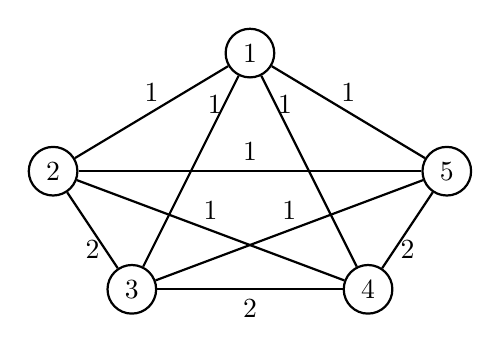
\begin{tikzpicture}[node distance={15mm}, thick, main/.style = {draw, circle}]
% [->,>=stealth,shorten >=1pt,auto,node distance=3cm,
%                         thick,main node/.style={circle,draw,font=\sffamily\Large\bfseries}]
    \node[main] (1) at (1.5,6) {1};
    \node[main] (2) at (-1,4.5) {2};
    \node[main] (3) at (0,3) {3};
    \node[main] (4) at (3,3) {4};
    \node[main] (5) at (4,4.5) {5};

\draw (1) -- (2) node[midway, above] {1};
\draw (1) -- (3) node[near start, above] {1};
\draw (1) -- (4) node[near start, above] {1};
\draw (1) -- (5) node[midway, above] {1};
\draw (2) -- (3) node[midway, below] {2};
\draw (3) -- (4) node[midway, below] {2};
\draw (4) -- (5) node[midway, below] {2};
\draw (4) -- (2) node[midway, above] {1};
\draw (3) -- (5) node[midway, above] {1};
\draw (2) -- (5) node[midway, above] {1};

\end{tikzpicture}

Presupunem ca algoritmul nostru va considera urmatorul $MST$\\

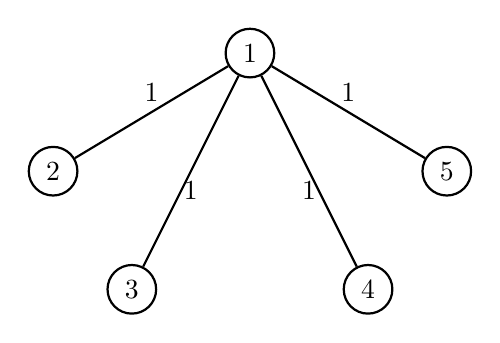
\begin{tikzpicture}[node distance={15mm}, thick, main/.style = {draw, circle}]
% [->,>=stealth,shorten >=1pt,auto,node distance=3cm,
%                         thick,main node/.style={circle,draw,font=\sffamily\Large\bfseries}]
    \node[main] (1) at (1.5,6) {1};
    \node[main] (2) at (-1,4.5) {2};
    \node[main] (3) at (0,3) {3};
    \node[main] (4) at (3,3) {4};
    \node[main] (5) at (4,4.5) {5};

\draw (1) -- (2) node[midway, above] {1};
\draw (1) -- (3) node[midway, below] {1};
\draw (1) -- (4) node[midway, below] {1};
\draw (1) -- (5) node[midway, above] {1};
\end{tikzpicture}

Considerand ca algoritmul din curs nu face nicio optimizare in ordinea in care selecteaza nodurile din $MST$,
algoritmul nostru poate considera ca solutie pentru TSP urmatorul ciclu:\\

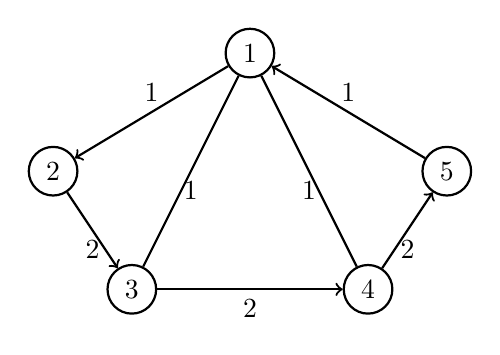
\begin{tikzpicture}[node distance={15mm}, thick, main/.style = {draw, circle}]
    \node[main] (1) at (1.5,6) {1};
    \node[main] (2) at (-1,4.5) {2};
    \node[main] (3) at (0,3) {3};
    \node[main] (4) at (3,3) {4};
    \node[main] (5) at (4,4.5) {5};

\draw[->] (1) -- (2) node[midway, above] {1};
\draw (1) -- (3) node[midway, below] {1};
\draw (1) -- (4) node[midway, below] {1};
\draw[->] (5) -- (1) node[midway, above] {1};
\draw[->] (2) -- (3) node[midway, below] {2};
\draw[->] (3) -- (4) node[midway, below] {2};
\draw[->](4) -- (5) node[midway, below] {2};
\end{tikzpicture}

Deci $ALG=len(1,2,3,4,5,1)=1+2+2+2+1=8$

Dar observam ca in cazul grafului $G$, solutia $OPT$ este:

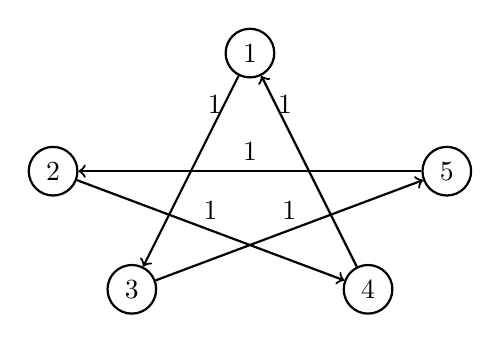
\begin{tikzpicture}[node distance={15mm}, thick, main/.style = {draw, circle}]
    \node[main] (1) at (1.5,6) {1};
    \node[main] (2) at (-1,4.5) {2};
    \node[main] (3) at (0,3) {3};
    \node[main] (4) at (3,3) {4};
    \node[main] (5) at (4,4.5) {5};

\draw[->] (1) -- (3) node[near start, above] {1};
\draw[->] (3) -- (5) node[midway, above] {1};
\draw[->] (5) -- (2) node[midway, above] {1};
\draw[->] (2) -- (4) node[midway, above] {1};
\draw[->] (4) -- (1) node[near end, above] {1};
\end{tikzpicture}

Deci $OPT=len(1,3,5,2,4,1)=1+1+1+1+1=5$\\

Deci avem ca:
\[ALG\leq \frac{3}{2}OPT \Leftrightarrow ALG=8\leq \frac{3}{2}OPT = \frac{3}{2}5 = 7.5 \Leftrightarrow 8\leq 7.5\]

Deci avem ca $ALG> \frac{3}{2}OPT$, adica $ALG$ nu este $\frac{3}{2}$ aproximativ.

\chapter*{Vertex Cover}
\addcontentsline{toc}{chapter}{Vertex Cover}
\setcounter{section}{0}

\section{Problema 1}

Deci avem $X=\{x_{1},x_{2}\dots x_{n}\}$ multimea variabilelor de tip bool si $C=\{C_{1},C_{2}\dots C_{m}\}$ cele m clauze si algoritmul:

\begin{tabbing}
\hspace{2em}
\= \kill Greedy-3CNF($C$, $X$)\\
1: $C=\{C_{1}\dots C_{m}\}$ mulțimea de predicate, $X=\{x_{1}\dots x_{n}\}$ - mulțime de variabile\\ 
2: cât timp $C\neq \emptyset$ execută\\ 
\> 3: Alegem aleator $C_{j}\in C$.\\
\> 4: Fie $x_{i}$ una dintre variabilele din $C_{j}$ .\\
\> 5: $x_{i}\leftarrow$ true.\\
\> 6: Eliminăm din $C$ toate predicatele ce îl conțin pe $x_{i}$ .\\
7: return $X$\\
\end{tabbing}


\subsection{}

In cazul algoritmului nostru consideram ca $\exists$ o var $x_{1}$ care se afla in toate $C_{i}, i=\overline{1,m}$ si in rest valori unice $x_{C_{i1}}$ si $x_{C_{i2}}$ pentru fiecare $C_{i}, i=\overline{1,m}$.

In acest caz algoritmul nostru poate sa selecteze toate variabilele ignorand $x_{1}$, deci problema care are $OPT=1$, algoritmul nostru poate fi $ALG=2m$, adica nu are o aproximare fixa, si poate lua valori foarte mari.\\

Deci factorul de aproximare worst case este $ALG=2mOPT$

\subsection{}

Pentru a obtine un algoritm 3-aproximativ trebuie sa modificam linia 4, sa faca toate valorile $x_{i}=1, x_{i} \in C_{j}$

\begin{tabbing}
\hspace{2em}\= \kill 
Greedy-3CNF($C$, $X$)\\
1: $C=\{C_{1}\dots C_{m}\}$ mulțimea de predicate, $X=\{x_{1}\dots x_{n}\}$ - mulțime de variabile\\ 
2: cât timp $C\neq \emptyset$ execută\\ 
\> 3: Alegem aleator $C_{j}\in C$.\\
\> 4: Pentru fiecare $x_{i} \in C_{j}$ .\\
\hspace{2em}\= \hspace{2em}\=)\kill 
\> \> 5: $x_{i}\leftarrow$ true.\\
\> \> 6: Eliminăm din $C$ toate predicatele ce îl conțin pe $x_{i}$ .\\
7: return $X$\\
\end{tabbing}

Acum trebuie sa demonstram ca $ALG\leq 3OPT$

La fiecare pas al algoritmului retinem in $P_{i}$ clauzele scoase din $C$. Sa presupunem ca sunt k pasi.\\

Deci $P_{i}=\{C_{j}\in C \mid C_{j}\text{ a fost scos la pasul i}\}$ 

Notam $P=\{P_{i} \mid i=\overline{1,k}\}$

Este evident ca $P$ este o partitie peste $C$, adica $\nexists$ 2 clauze comune intre oricare $P_{i}, P_{j}$ si $\bigcup\limits_{i=1}^{k} P_{i}=C$.

Deci observam ca intre oricare 2 multimi $P_{i}, P_{j}; \exists C_{a}\in P_{i} \text{ si } C_{b}\in P_{j}$ astfel incat $C_{a} \text{ si } C_{b}$ nu au niciun x in comun.

Asadar, optimul $OPT\geq \vert P\vert$ deoarece in cel mai bun caz $\forall P_{i}\in P$ necesita doar un $x_{i}=1$.

Evdent $ALG=3\cdot \vert P \vert$ (adica 3* numarul de pasi al algoritmului in care facem cate 3 variabile 1).

Asadar

\[ALG=3\cdot \vert P\vert \leq 3OPT \implies ALG\leq 3OPT\]

\subsection{}
Ca sa traducem in programare liniara considerm urmatoarea situatie in programare liniara 0/1, care e chivalenta cu problema 3CNF:

\begin{tabbing}
\hspace{2em}\= \kill 
minimizam $\sum_{i=1}^{n}x_{i}$ \\
a.i. \> $x_{a}+x_{b}+x_{c}\geq 1 \text{ unde } x_{a},x_{b},x_{c}\in C_{i}, i=\overline{1,m}$ \\
\> $x_{i}\in \{0, 1\}$
\end{tabbing}
Notam $OPT_{lin_{0/1}}$ rezultatul acestei probleme de programare liniara 0/1 si fie $OPT$ optimul pentru 3CNF. Observam ca:

\[OPT_{lin_{0/1}}=OPT\]

Dar problema de programare liniara 0/1 prezentata mai sus este NPC. Deci vom face o relaxare a problemei pentru a o duce in programare liniara cu numere reale. 
Notam cu $x'_{i}$ valoarea lui $x_{i}$ dusa in intervalul $[0,1]$, adica $x'_{i}\in [0,1]$

Deci acum avem:

\begin{tabbing}
\hspace{2em}\= \kill 
minimizam $\sum_{i=1}^{n}x'_{i}$ \\
a.i. \> $x'_{a}+x'_{b}+x'_{c}\geq 1 \text{ unde } x_{a},x_{b},x_{c}\in C_{i}, i=\overline{1,m}$ \\
\> $0\leq x'_{i}\leq 1$
\end{tabbing}

Fie $OPT_{lin}$ valoarea sumei $\sum_{i=1}^{n}x'_{i}$ in urma rezolvarii problemei de programare liniara prezentata mai sus.
Observam ca $OPT_{lin}\leq OPT_{lin_{0/1}}$ deoarece noi am facut o relaxare a constrangerilor variantei 0/1, adica este cel putin la fel de buna ca ea.

Adica cum $OPT_{lin_{0/1}}=OPT$, obtinem:

\[OPT_{lin}\leq OPT\]

Acum avem algoritmul pentru problema 3CNF:

\begin{tabbing}
Prog-liniara-3CNF($C$, $X$)\\
1: $X=\{x_{1}\dots x_{n}\}$ - mulțime de variabile, $X'=\{x'_{1}\dots x'_{n}\}$ - variabilele $\in [0,1]$ \\ 
2: Rezolva urmatoarea problema de programare liniara:\\
\hspace{2em}\= \kill 
3: \> minimizam $\sum_{i=1}^{n}x'_{i}$ \\
\hspace{2em}\=\hspace{2em}\= \kill 
\> a.i. \> $x'_{a}+x'_{b}+x'_{c}\geq 1 \text{ unde } x_{a},x_{b},x_{c}\in C_{i}, i=\overline{1,m}$ \\
\> \> $0\leq x'_{i}\leq 1$\\
\hspace{2em}\=\kill 
4: $X=\{x_{i}=1 \mid x'_{i}\geq \frac{1}{3}\}$\\
5: return X
\end{tabbing}

\subsection{}

In primul rand trebuie sa demonstram ca toate clauzele $C_{i}\in C$ sunt satisfacute.

Acest lucru reiese din constrangerea $x'_{a}+x'_{b}+x'_{c}\geq 1$, adica cel putin o variabila este $\geq \frac{1}{3}$
adica ia o valoare finala 1, asta pentru fiecare $C_{i}\in C$. Deci algoritmul rezolva corect problema 3CNF.

Acum trebuie sa demonstram ca $ALG\leq 3OPT$

Este evident ca $ALG=\sum_{i=1}^{n}x_{i}$\\

Deci avem ca \[OPT_{lin}=\sum_{i=1}^{n}x'_{i}\]

Si stim ca $OPT_{lin}\leq OPT$ si $x'_{i}\geq \frac{1}{3}$ pentru orice $x_{i}$ care are valoarea 1 la final. Deci:

\[ALG=\sum_{i=1}^{n}x_{i}\leq 3\cdot \sum_{i=1}^{n}x'_{i}\leq 3\cdot OPT_{lin} \leq 3\cdot OPT\]

Deci avem ca algoritmul nostru este 3-aproximativ:

\[ALG\leq 3OPT\]

\end{document}

